\section{Aufbau und Durchführung}
\label{sec:Durchführung}

\subsection{Justage}
Zu Beginn ist eine Justierung des Interferometers notwendig.
Ziel ist eine Aufspaltung eines Strahls in Zwei Strahlen, die beide in
der horizonthalen Ebene liegen und anschließendes Überlappen der Strahlen
beim Verlassen des Interferometers. Dies wird durch Einstellen der
Spiegel innerhalb und außerhalb des Interferometers erreicht.

Die  Apperatur ist aufgebaut wie in Abbildung \ref{fig:apparat}.
\begin{figure}
    \centering
    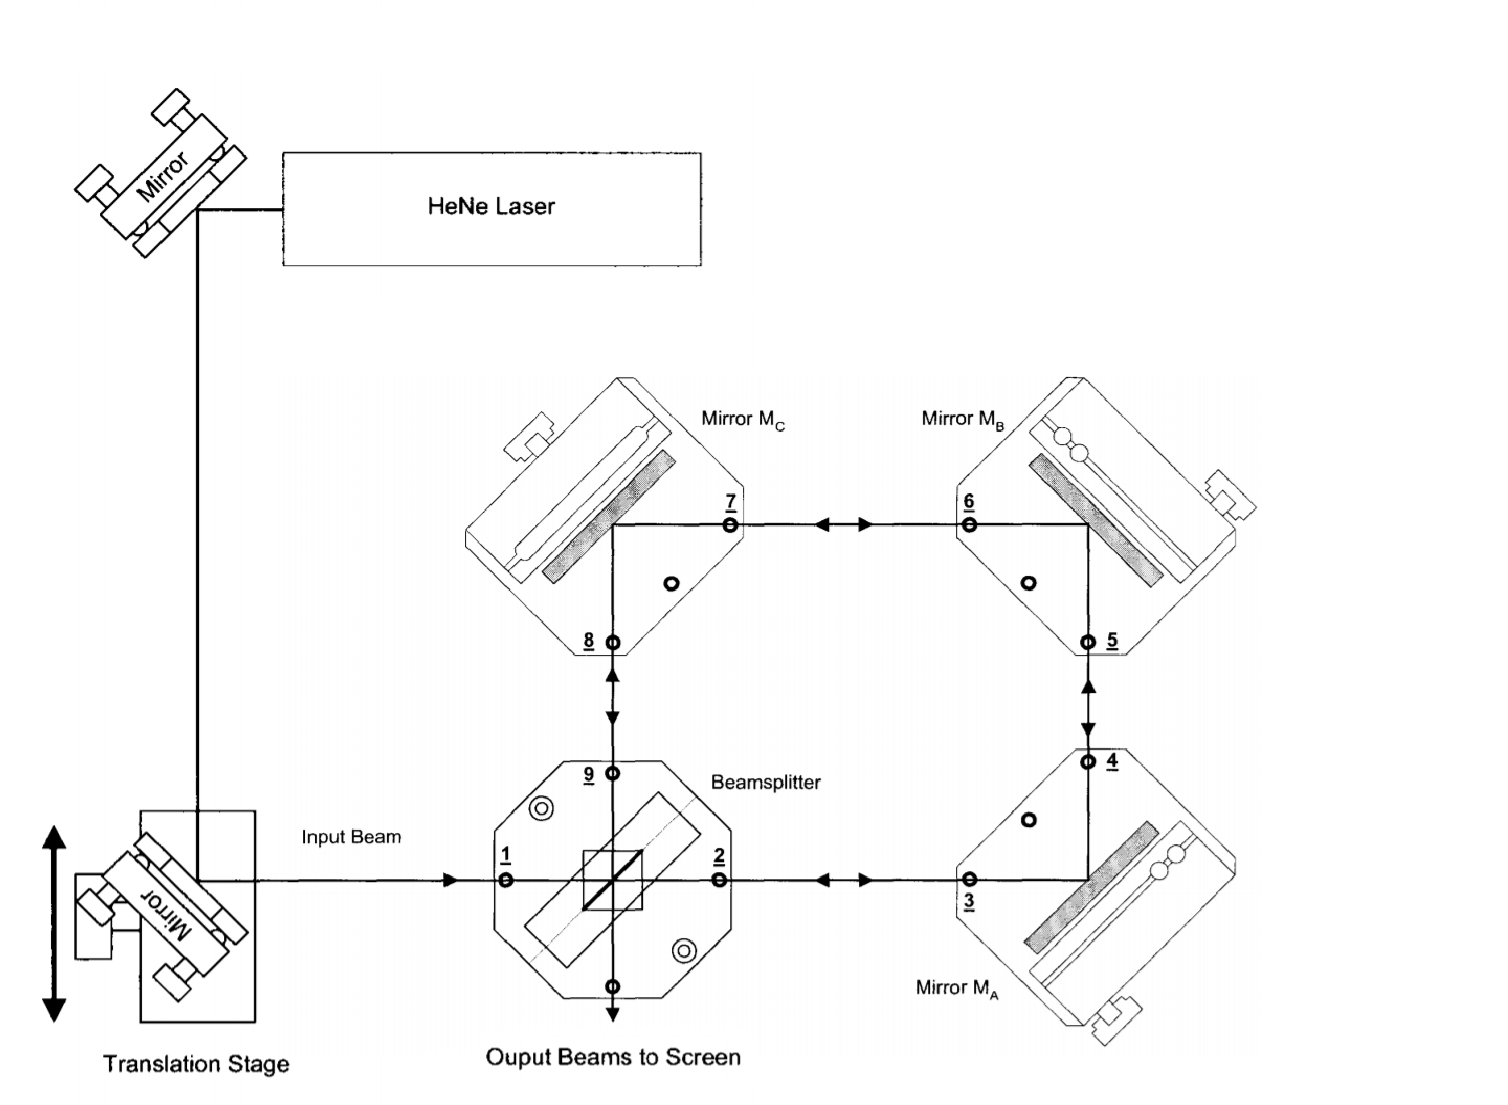
\includegraphics[width=0.7\textwidth]{Apperatur.PNG}
    \caption{Aufbau des Sagnac-Interferometers.\cite{skript}}
    \label{fig:apparat}
\end{figure}
Die Anordnung setzt sich zusammen aus der Quelle, einem HeNe-Laser, zwei
Spiegel zur Ausrichtung des Laserstrahls zum Polarizing-Beam-Splitter-Cube hin.
Zuvor passiert der Laserstrahl einen linearen Polarisationsfilter.
Der PBSC dient zur Aufspaltung des Strahls in Horizntal-und Vertikalkomponente,
dabein passiert die Horizontalkomponente den PBSC und die Vertikalkomponente wird
erfährt einen Richtungsänderung um $90\si{\degree}$. Drei weitere Spiegel lenken
beide Strahle so um, dass diese die gleiche Strecke zurücklegen und wieder auf
den PBSC treffen. Dort werden die Strahlen erneut, nach ihrer polarisation,
umgelenkt und durchgelassen, somit laufen die Strahlen wieder zusammen.
Durch verschieben der Translation Stage können die zwei Strahlen räumlich separiert
werden und somit unterschiedliche Materialien durchqueren.
Bei der ersten Messung werden zwei Glasplättchen, die auf einer Rotationsachse
befestigt sind, unterschiedlicher
Ausrichtung in die beiden Strahlengänge positioniert, zu sehen in der Abbildung
\ref{fig:glasplattchen}.

\begin{figure}
     \centering
     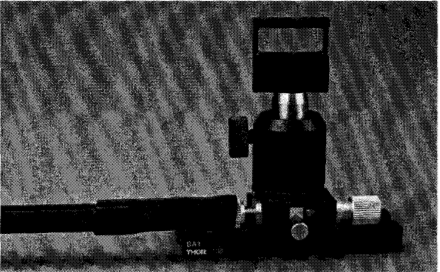
\includegraphics[width=0.7\textwidth]{Glasblattchen.PNG}
     \caption{Rotationsachse mit Glasblättchen.\cite{skript}}
     \label{fig:glasplattchen}
\end{figure}
Zur Messung des Kontrasts wird ein linearer Polarisationsfilter mit $45\si{\degree}$
Ausrichtung verwendet, der hinter dem PBSC positioniert wird.
Dadurch entsteht ein Interferenzbild, dessen Intensität durch eine Photodiode gemessen wird.
Nun wird der Winkel des ersten Polarisationsfilters variiert
und die Glasplättchen so rotiert, dass einmal ein Intensität minima und einmal
ein Intensitäts maxima gemessenwerden kann.

Für die Bestimmung der Brechungsindexe wird der
Winkel des ersten Polarisationsfilters so gewählt, dass ein Kontrast Maximum vorliegt.
des weiteren wird der zweite Polatriationsfilter und die Photodiode entfern.
Statdessen trifft der gebündelte Strahl nun einen Polarisationsseperator realisiert durch einen
weiteren PBSC und einen Spiegel, wie in Abbildung \ref{fig:polsep} zu sehen.
\begin{figure}
     \centering
     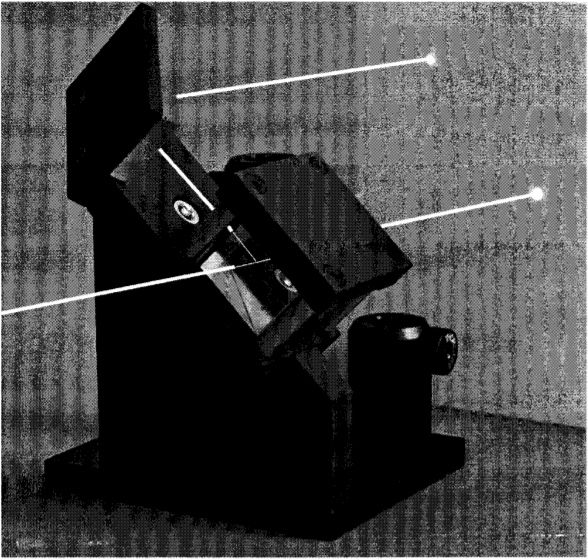
\includegraphics[width=0.7\textwidth]{PSBC.PNG}
     \caption{Aufbau des Polarisationsseperator.\cite{skript}}
     \label{fig:polsep}
\end{figure}

Mittels zweier Photodioden wird der zuvor aufgespaltene Strahl detektiert.
Mit einem Oszilloskop wird die Spannungsdifferenz zwischen den Intensitäten
gemessen. Ein weiteres Gerät zähl die Nulldurchgänge der Spannungsdifferenz.
Bei der Messung für den Brechungsindex von Glas wird
der Winkel der Glasplättchen langsam verändert und die Nulldurchgänge für unterschiedliche
winkel aufgenommen.

Für den Brechnungsindex von Luft werden die Glasplättchen
aus dem Strahlengang enfernt. Es wird eine Gaszelle eingebaut, durch
die nur ein Laserstrahl geht. Die Gaszelle ist verbunden mit einer Pumpe
die ein Vakuum in der Gaszelle erzeugt. Durch ein Ventil wird wieder langsam
Luft in die Zelle gelassen bis wieder der Normaldruck erreicht ist. Während
dieses Vorganges werden wieder Nulldurchgänge von der Spannungsdifferenz aufgenommen.
